% *** Equilibrium ***
\chapter{Equilibrium}
\section{Homework: Equilibrium}
\subsection{Dissociation}
\subsubsection{Problem}
Consider the following aqueous equilibrium,
where \(\Delta H = +\qty{45.3}{kJ.mol^{-1}}\)
\sidenote{This is an endothermic reaction!}:
\begin{equation}
	\ch{HOCl \aq{} <=> H+ \aq{} + OCl- \aq}
	\label{eq:hocl}
\end{equation}

The \hil{concentrations} of the three species were recorded over time as shown:
\begin{figure}[htpb]
	\centering
	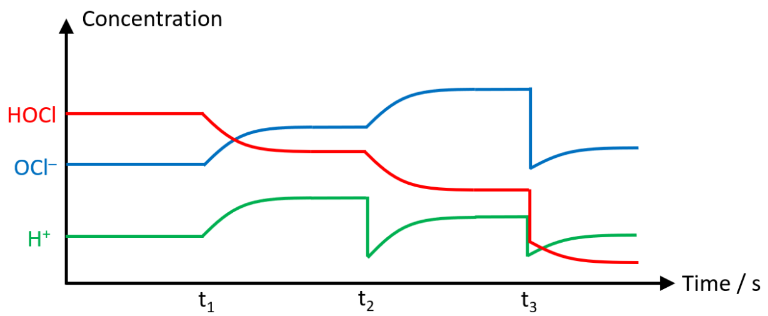
\includegraphics[width=0.80\linewidth]{assets/07_hocl_concentrations.png}
	\caption{Concentrations of \ch{H^{+}}, \ch{OCl-} and \ch{HOCl} against time}
	\label{fig:hocl}
\end{figure}

Suggest the changes necessary at \(t_1\), \(t_2\) and \(t_3\) to produce the
above graph.

\subsubsection{Solution}

We can write
\begin{equation}
	K_c = \frac{\ch{[H^{+}]} \ch{[OCl^-]}}{\ch{[HOCl]}}
	\label{eq:hocl-kc}
\end{equation}

\begin{itemize}
	\item At \(t_1\), \ch{[HOCl]} drops and \ch{[H^{+}]} and \ch{[OCl^-]} rises. \(K_c\)
	      rises. The equilibrium position is moved to the right, and {\color{accent} the
			      temperature of the solution has been increased}.
	\item At \(t_2\), \ch{[HOCl]} continues to drop gradually, \ch{[H^{+}]} drops sharply
	      and \ch{[OCl^-]} increases gradually. It is expected that both \ch{[H^{+}]} and \ch{[OCl]}
	      would continue rising under, for example, an increase in temperature, but
	      the significant drop in \ch{[H^{+}]} suggests the removal of \ch{H+} ions.
	      Therefore, {\color{accent} a strong base (e.g. \ch{NaOH \aq}) had been added},
	      which neutralised \ch{H+} while shifting the equilibrium position to the right
	      to continue producting \ch{OCl-}.
	\item At \(t_3\), \ch{[HOCl]}, \ch{[OCl^-]} and \ch{[H^{+}]} all drop drastically. However,
	      \ch{[HOCl]} continues decreasing and \ch{[H^{+}]} and \ch{[OCl^-]} continue increasing (albeit
	      at a lower rate) after \(t_3\), suggesting that {\color{accent} the solution had been
			      diluted with \ch{H2O \lqd}}.
\end{itemize}

\subsection{Trouble concentrating}
\subsubsection{Problem}

In the reaction below, \qty{4.0}{\mol} \ch{H2} and \qty{2.0}{\mol} \ch{I2} are allowed
to react in a \qty{2.0}{\dm\cubed} vessel at \qty{440}{\celsius}.
\begin{equation}
	\ch{H2 \gas{} + I2 \gas{} <=> 2 HI \gas}
\end{equation}
The equilibrium concentration of \ch{HI} is \qty{1.9}{\conc}.

Calculate the \(K_c\) for the reaction\sidenote{equilibrium constant} at
\qty{440}{\celsius}, stating its units.

\subsubsection{Solution}
\begin{align*}
	\eta_{\ch{HI}}                                                                & = \qty{1.9}{\mol\per\dm\cubed} \times \qty{2.0}{\dm\cubed}                                      \\
	                                                                              & = \qty{3.8}{\mol}                                                                               \\
	\\
	\eta_{\ch{H2}} \text{ reacted}                                                & = \slf{\qty{3.8}{\mol}}{ 2                                                                    } \\
	                                                                              & = \qty{1.9}{\mol}                                                                               \\
	\because \eta_{\ch{H2}} \text{ reacted} \colon \eta_{\ch{I2}} \text{ reacted} & = 1 \colon 1                                                                                    \\
	\eta_{\ch{H2}} \text { at eq.}                                                & = \qty{4.0}{\mol} - \qty{1.9}{\mol} = \qty{2.1}{\mol}                                           \\
	\eta_{\ch{I2}} \text { at eq.}                                                & = \qty{2.0}{\mol} - \qty{1.9}{\mol} = \qty{0.1}{\mol}                                           \\
	\\
	\ch{[H2]}                                                                     & = \slf{\qty{2.1}{\mol}}{\qty{2.0}{\dm\cubed}} = \qty{1.05}{\conc}                               \\
	\ch{[I2]}                                                                     & =  \slf{\qty{0.1}{\mol}}{\qty{2.0}{\dm\cubed}} = \qty{0.05}{\conc}                              \\
	\\
	K_c                                                                           & = \frac{\ch{[HI]}^2}{\ch{[H2]} \ch{[I2]}}                                                       \\
	                                                                              & = \frac{\ab(\qty{1.9}{\mol\per\dm\cubed})^2}{\qty{1.05}{\conc} \times \qty{0.05}{\conc}}        \\
	                                                                              & = \color{accent} \num{68.8}
\end{align*}

\subsection{Under pressure}
\subsubsection{Problem}
A sample of pure \ch{NO2 \gas{}} when heated to \qty{1000}{\celsius} decomposes
according to the following equation (Equation~\ref{eq:no2-decomp}):
\begin{equation}
	\ch{2 NO2 \gas{} <=> O2 \gas{} + 2 NO \gas}
	\label{eq:no2-decomp}
\end{equation}
The equilibrium constant \(K_p\) is \qty{158}{\atm}. Analysis shows that the
partial pressure of oxygen is \qty{0.25}{\atm} at equilibrium.

Calculate the partial pressures of \ch{NO} and \ch{NO2} in the equilibrium
mixture.

\subsubsection{Solution}
\begin{align*}
	K_p                              & = \frac{P_{\ch{O2}}{P_{\ch{NO}}}^2}{{P_{\ch{NO2}}}^2}             \\
	\qty{158}{\atm}                  & = \qty{0.25}{\atm} \times \ab(\frac{P_{\ch{NO}}}{P_{\ch{NO2}}})^2 \\
	\frac{P_{\ch{NO}}}{P_{\ch{NO2}}} & = \sqrt{632}
\end{align*}

Let the change in the partial pressure of \ch{NO2} be \(p\), and the initial
pressure be \(P\).

We can construct an ICE table (Table~\ref{tab:no2-decomp}).
\begin{table}[htpb]
	\centering
	\begin{tabular}{l r r r}
		\toprule
		\textbf{Pressure / \unit{\atm}} & \textbf{\ch{NO2}} & \textbf{\ch{O2}} & \textbf{\ch{NO}} \\
		\midrule
		Initial                         & \(P\)             & 0                & 0                \\
		Change                          & \(-p\)            & \(+\slf{p}{2}\)  & \(+p\)           \\
		End                             & \(P-p\)           & \(\slf{p}{2}\)   & \(p\)            \\
		\bottomrule
	\end{tabular}
	\caption{ICE table for the decomposition of \ch{NO2}}
	\label{tab:no2-decomp}
\end{table}

Given that the partial pressure of \ch{O2} is \qty{0.25}{\atm} at equilibrium,
\begin{align*}
	\slf{p}{2}                 & = \qty{0.25}{\atm}                \\
	P_{\ch{NO}} = p            & = \color{accent} \qty{0.50}{\atm} \\
	P_{\ch{NO2}} = p\sqrt{632} & = \color{accent} \qty{12.6}{\atm}
\end{align*}

\subsection{Silver salts}
\subsubsection{Problem}
Silver(I) chloride (\(K_{\text{sp}} = \num{1.82e-10}\) at \qty{298}{\kelvin}) is
a sparingly soluble salt. Silver(I) chromate(VI), \ch{Ag2CrO4}, is another
sparingly soluble salt, with \(K_{\text{sp}} = \num{1.18e-12}\) at
\qty{298}{\kelvin}.

\begin{enumerate}
	\item Calculate the solubility of silver(I) chloride in water at \qty{298}{\kelvin}.
	\item Show that \ch{Ag2CrO4} is \textbf{more} soluble in water than \ch{AgCl} at
	      \qty{298}{\kelvin} although the value of \(K_{\text{sp}}\) is smaller than
	      that of \ch{AgCl}.
\end{enumerate}

\subsubsection{Solution}
The dissolution of silver(I) chloride can be written as
\begin{equation}
	\ch{AgCl \sld{} <=> Ag+ \aq{} + Cl- \aq}
	\label{eq:agcl}
\end{equation}

We can thus say\sidenote{\ch{AgCl} is a solid, so there is no denominator.}

\begin{align*}
	K_{\text{sp}} & = \ch{[ Ag^{+} ]} \ch{[Cl^-]}
\end{align*}

Let the solubility of \ch{AgCl \sld} be \(S\).

\begin{align*}
	S = \ch{[AgCl]}                             & = \ch{[ Ag^{+} ]} = \ch{[Cl^-]}       \\
	K_{\text{sp}} = \ch{[ Ag^{+} ]} \ch{[Cl^-]} & = S \times S = S^2                    \\
	S                                           & = \sqrt{\num{1.82e-10}}               \\
	                                            & = \color{accent} \qty{1.35e-5}{\conc}
\end{align*}

Let the solubility of \ch{Ag2CrO4} at \qty{298}{\kelvin} be \(S_1\). We can write
\begin{equation}
	\ch{Ag2CrO4 \sld{} <=> 2 Ag+ \aq{} + CrO4^{2-} \aq}
	\label{eq:ag2cro4}
\end{equation}
\begin{align*}
	S_1 = \ch{[CrO4^{2-}]} & = \slf{\ch{[Ag^{+}]}}{2}           \\
	K_{\text{sp}}          & = \ch{[Ag^{+}]}^2 \ch{[CrO4^{2-}]} \\
	                       & = 4{S_1}^3                         \\
	                       & = \num{1.18e-12}                   \\
	\\
	S_1                    & = \sqrt[3]{\f{\num{1.18e-12}}{4}}  \\
	                       & = \qty{6.66e-5}{\conc}             \\
	\\
	\therefore S_1         & > S \qed
\end{align*}
{\color{accent} \ch{Ag2CrO4} is more soluble than \ch{AgCl} in water at \qty{298}{\kelvin}.}
